\section{Conclusion}
\label{sec:concl}



 

In this work, we presented a comprehensive theoretical analysis of gradient-based learning in high-dimensional, extensive-width two-layer neural networks with quadratic activation.  We established precise scaling
laws that characterize both the population gradient flow and its empirical, discrete-time approximation.
These results demonstrate how anisotropic signal strengths in the target function fundamentally shapes the
convergence behavior and sample efficiency of gradient-based learning. 

\paragraph{Beyond quadratic activations.} 
An immediate direction for future research is to extend our analysis to more general activation functions. Link functions with higher information exponent is studied in a companion work \cite{ren2025emergence}, where the precise risk scaling is established by exploiting a decoupling structure that is unique to the information exponent $k>2$ setting. 
Importantly, many commonly-used activation functions (ReLU, GeLU, etc.) have information exponent $k=1$ and also contain a nonzero $\mathrm{He}_2$ component. For such nonlinearities, we conjecture that SGD dynamics exhibits a multi-phase risk curve (analogous to the incremental learning phenomenon in \cite{abbe2023sgd,bietti2023learning}), where the higher Hermite modes affects the learning dynamics after the low-order terms are learned. In Figure \ref{fig:scalinglaw-relu} we report the SGD risk curves for ReLU networks, in which we observe $(i)$ an initial loss drop driven by the $\mathrm{He}_1$ component (which finds a degenerate rank-1 subspace), followed by $(ii)$ a power-law decay phase driven by the quadratic $\mathrm{He}_2$ component where the empirical scaling exponent align closely with our theoretical predictions, and finally $(iii)$ a slope change late in training likely due to higher Hermite terms (in Figure~\ref{fig:scalinglaw-mixture} we confirm that this ``late'' phase is absent if we remove these higher-order components). Understanding such complex multi-phase learning dynamics remains an interesting challenge for future work. 

 


\begin{figure}[!htb]
  \begin{subfigure}{0.45\textwidth}
    \centering
    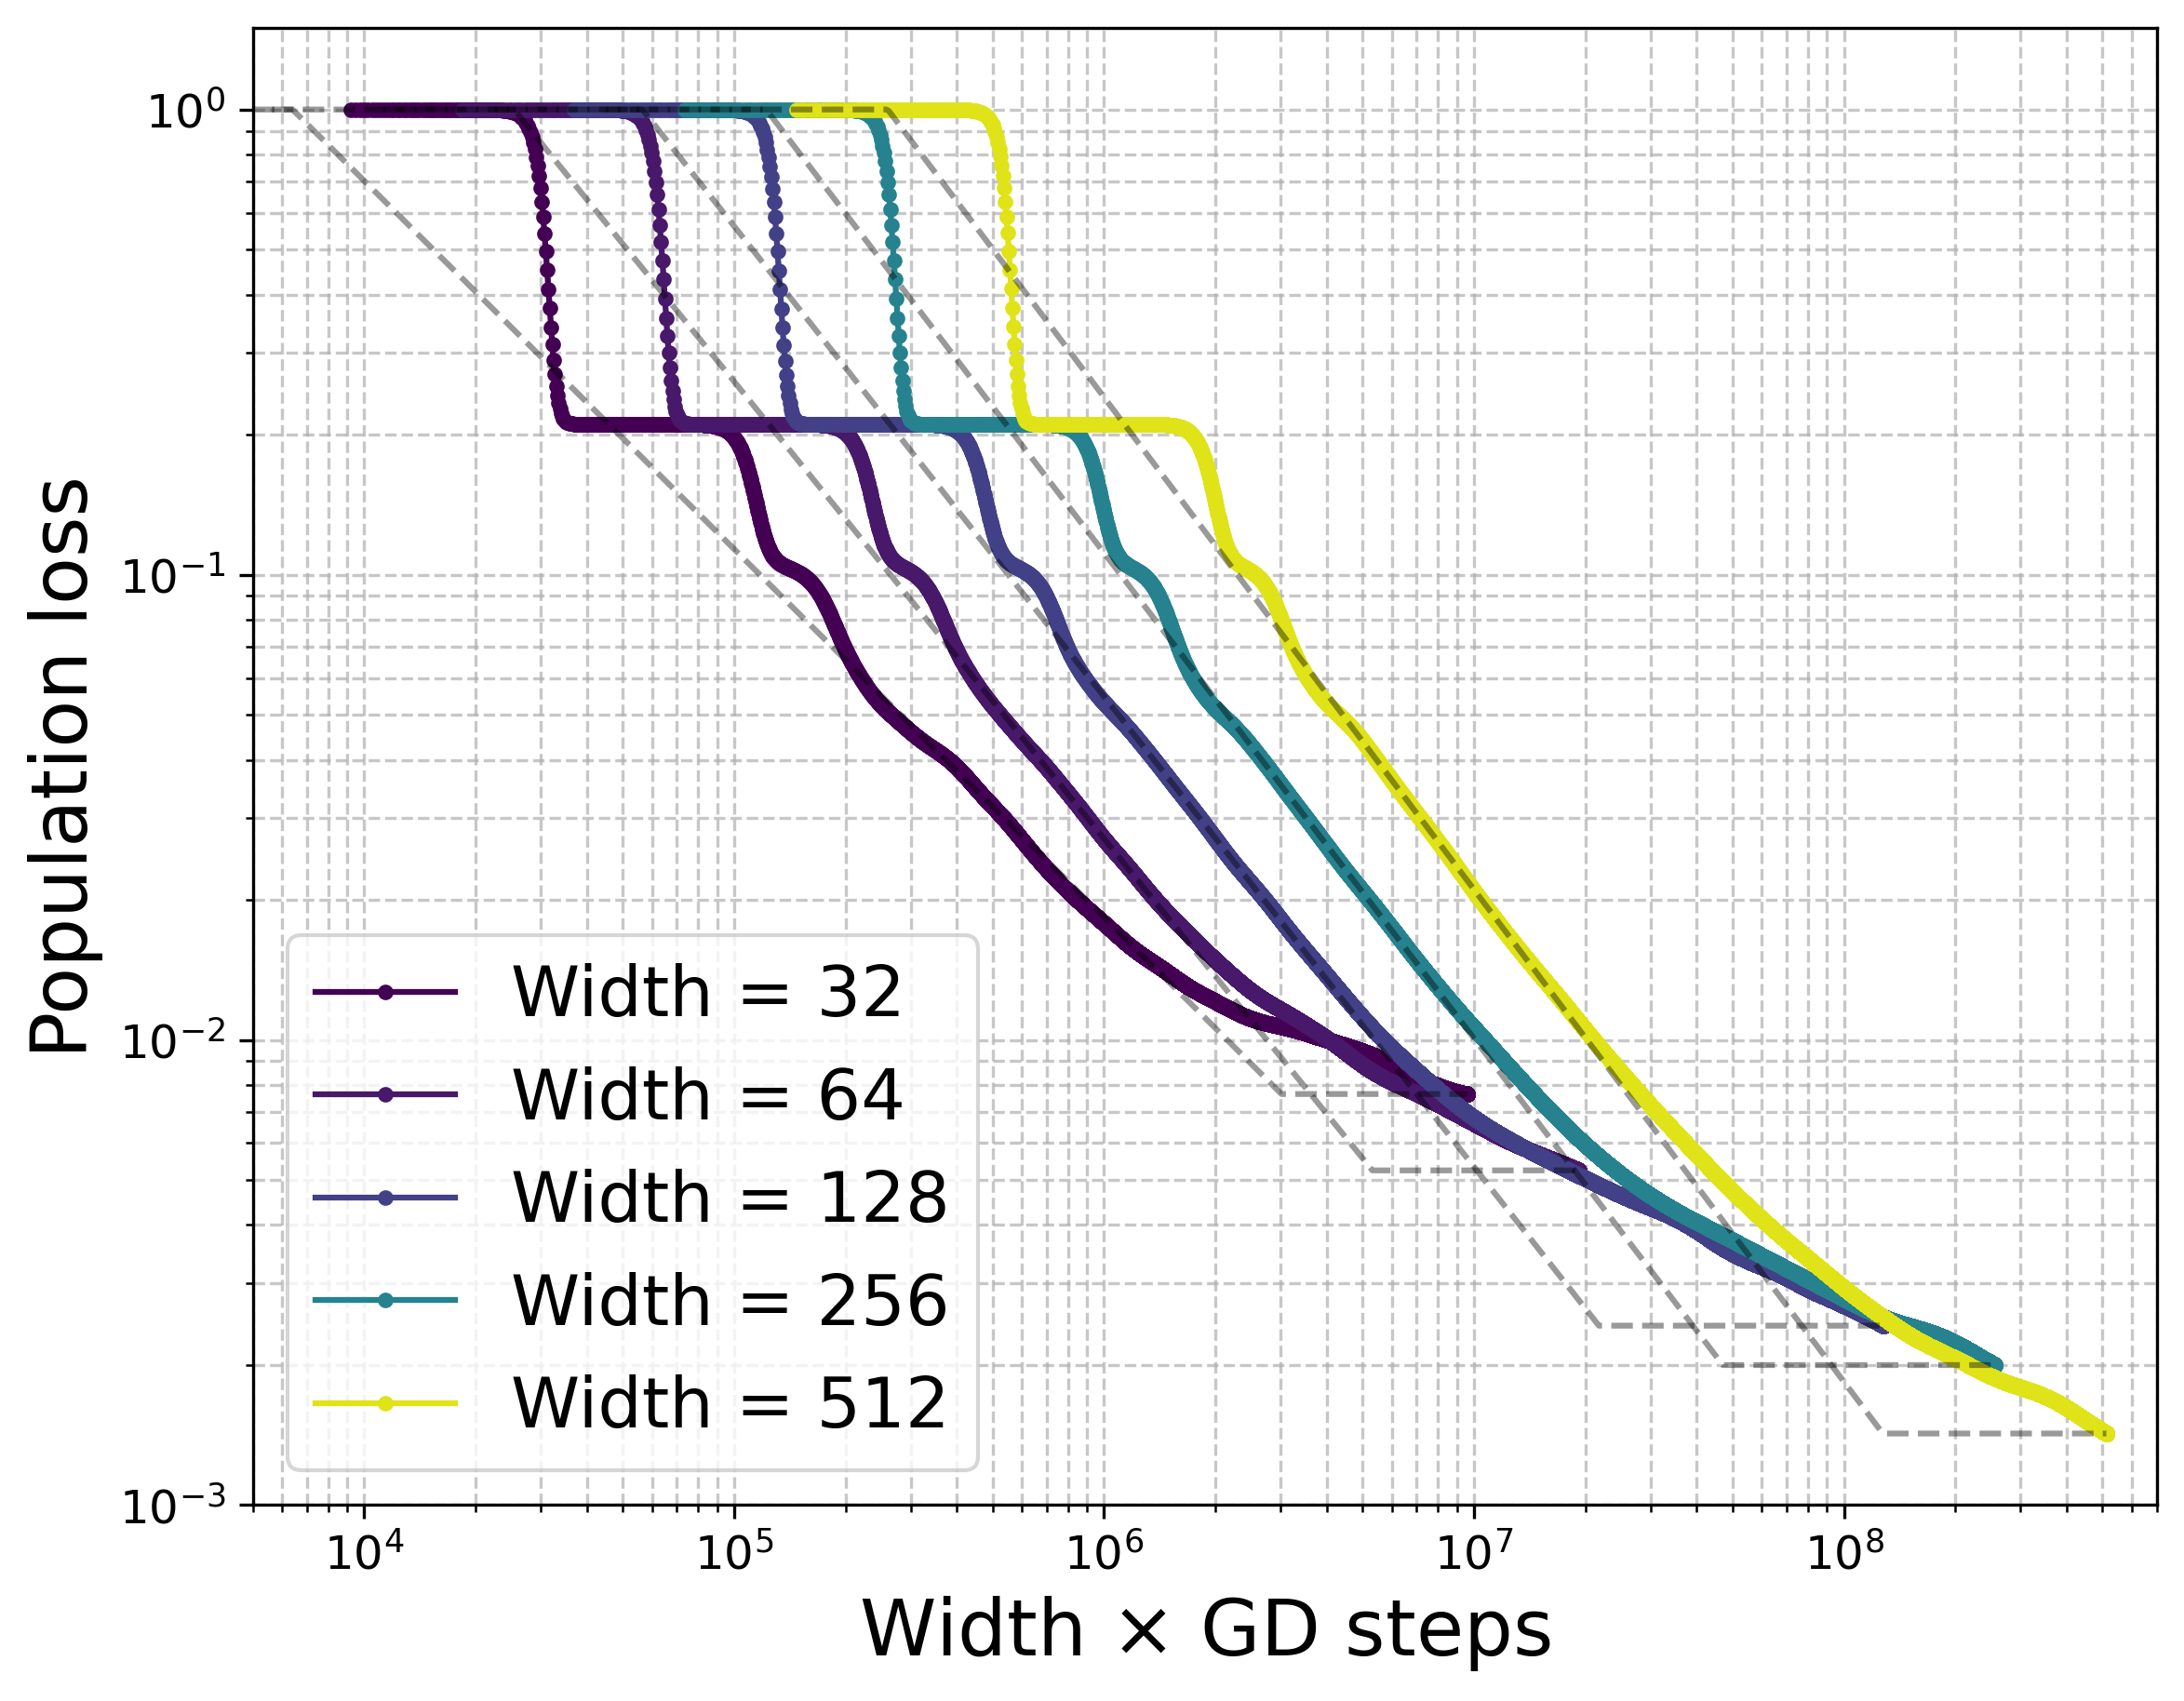
\includegraphics[width=0.95\textwidth]{_figures/__scaling_results_centered_relu_d5000_beta10_ext2.png}
    \caption{$\alpha = 1$. Ideal exponent: $-1$; empirical:  $-1.01$.\!\!}
    \label{fig:relua10}
  \end{subfigure}
   ~~~~~~\begin{subfigure}{0.45\textwidth}
   \centering
     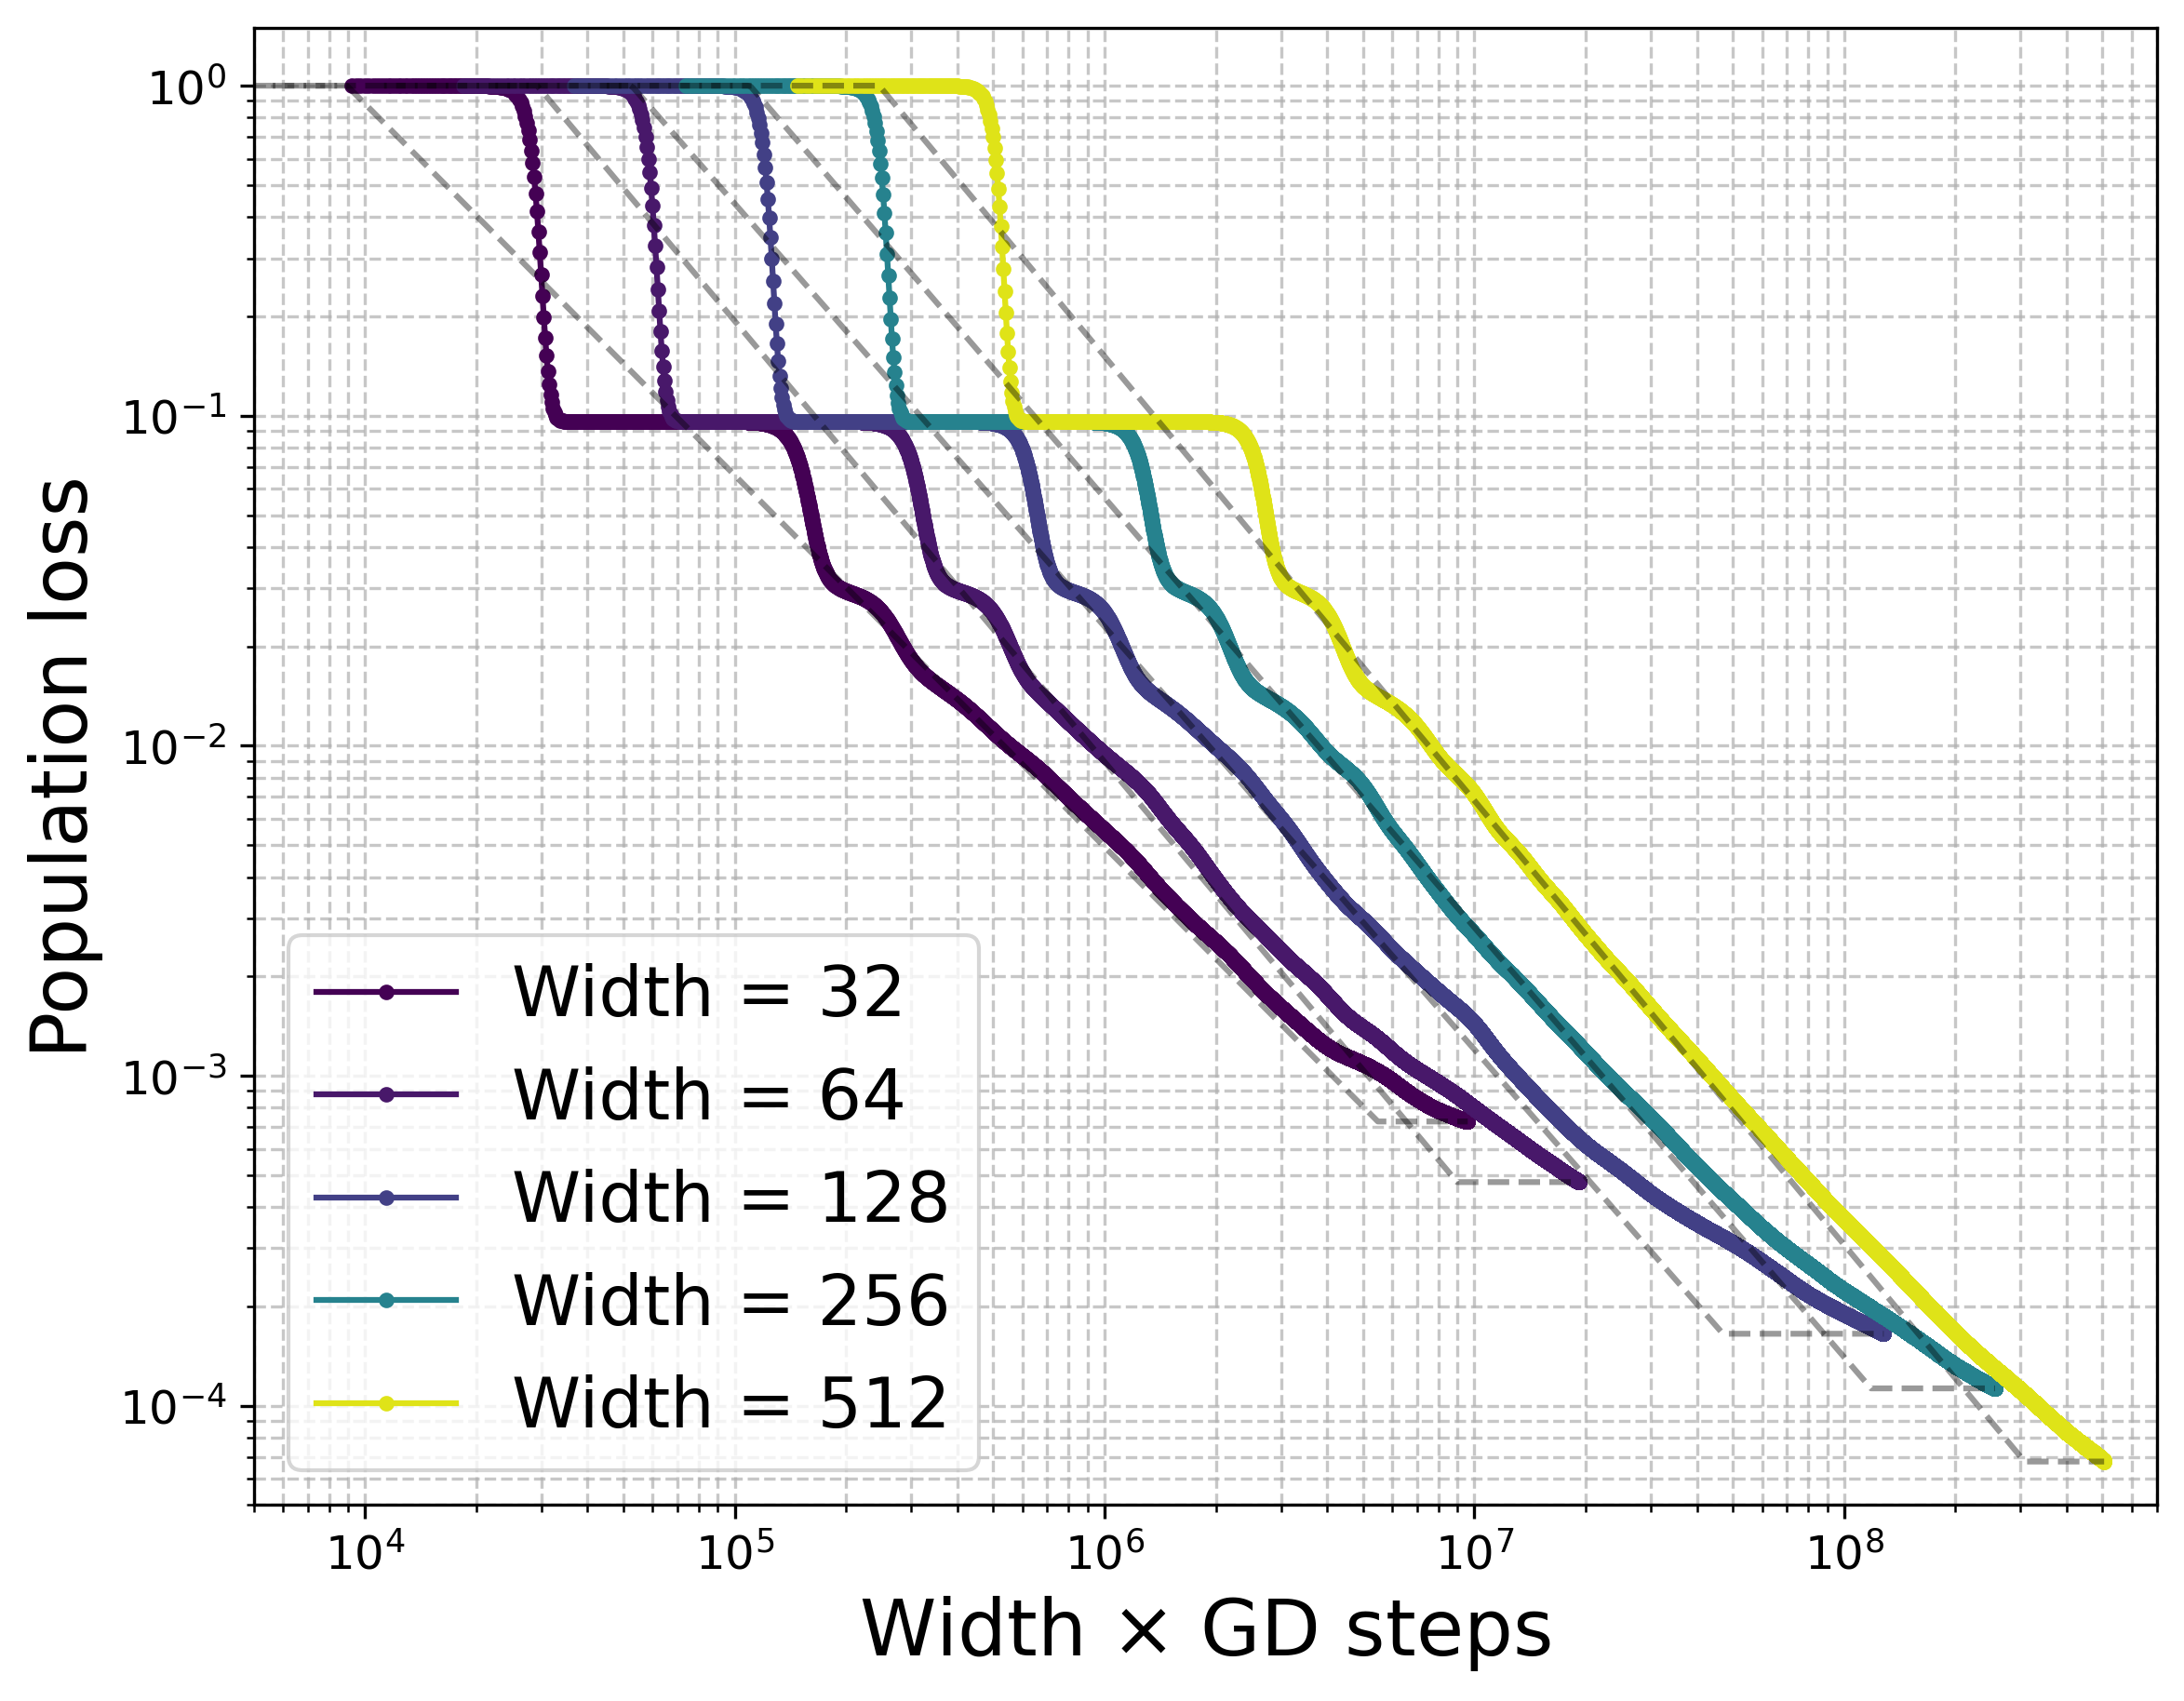
\includegraphics[width=0.95\textwidth]{_figures/__scaling_results_centered_relu_d5000_beta15_ext2.png}
     \caption{$\alpha = \frac{3}{2}$. Ideal exponent; $-\frac{4}{3}$, empirical:: $- 1.26$.\!\!}
    \label{fig:relua15}
    \end{subfigure} 
\caption{\small  Population loss vs.~compute for two-layer ReLU network (power-law second-layer with exponent $\alpha$) trained with population gradient descent. The student network adopts the 2-homogeneous parameterization as in \eqref{eq:student}. Observe that after the initial loss drop due to the $\mathrm{He}_1$ component, the risk curves follow a power-law scaling where the exponent (dashed lines) nearly matches our theoretical prediction for the quadratic setting $\frac{1-2\alpha}{\alpha}$.}
  \label{fig:scalinglaw-relu} 
% \vspace{-3mm}
\end{figure}

